\section{Machine Learning Models}
\label{sec:ML}

As price prediction is a common regression task, multiple regressors are trained seperately and the best performing 
models are ensembled using a VotingRegressor.

\subsection{Regression Models}

For the single regressor models, the models \textit{XGBoost} (one tree based, one based on linear models), \textit{CatBoost},
\textit{AdaBoost} and \textit{ExtraTrees} were trained and compared using the three scaling methods discussed in \autoref{sec:Expl}
and with no scaling.\\
The target variable \textit{Price} is scaled logarithmic. Training based on a Min-Max scaling of the price yielded worse results
on average. The training and testing split was done by using the train test split function of the sklearn.modelselection
library and set as $30 \, \% - 70 \, \%$ .\\
For the training of the individual models, a Pipeline, involving a \textit{preprocessor}, a \textit{feature selection} and the 
respective \textit{regressor}. The preprocessor consists of a numeric and categorical transformer. The numeric transformer uses 
a SimpleImputer to fill missing entries with the mean and also scales entries according to the chosen scaling method. The categorical
transformer suses a SimpleImputer to fill \texttt{NaNs} with the most frequent entry and handles categorical values
with a OneHotEncoder which creates dummy columns.\\
The feature selection is done with an Extra Trees Regressor, which evaluates the most important features, which are then used 
for the training. The hyperparameters are optimised by using a Randomised Search with 10-fold Cross Validation. The best parameters
for each scaling for each model can be found in the \autoref{sec:Appendix}.\\
As evaluation metrics, a 10-fold Cross Validation of the Root Mean Squared Error (RMSE) is performed and the Mean Squared Error (MSE),
Mean Absolute Error (MAE), $ \mathrm{R}^2 $ are evaluated for the test sub set and the Training Time (TT) is extracted. The results
are shown in \autoref{tab:Metrics}.
The most important parameters chosen by the ExtraTrees Regressor are visually represented in \autoref{fig:Most_Imp}.


\subsection{Ensembled Model}



\begin{figure}
\centering
    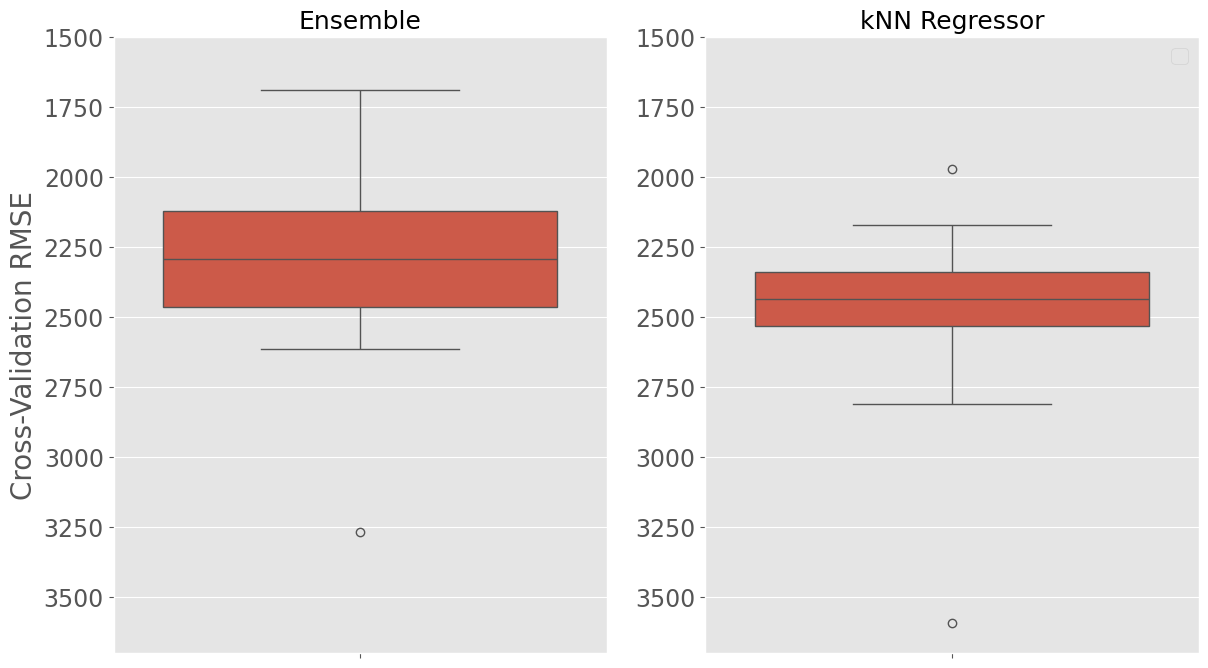
\includegraphics[width=0.9\textwidth]{"content/pics/boxplots_crossval.png"}
    \caption{.}
    \label{fig:}
\end{figure}



\begin{figure}
\centering
    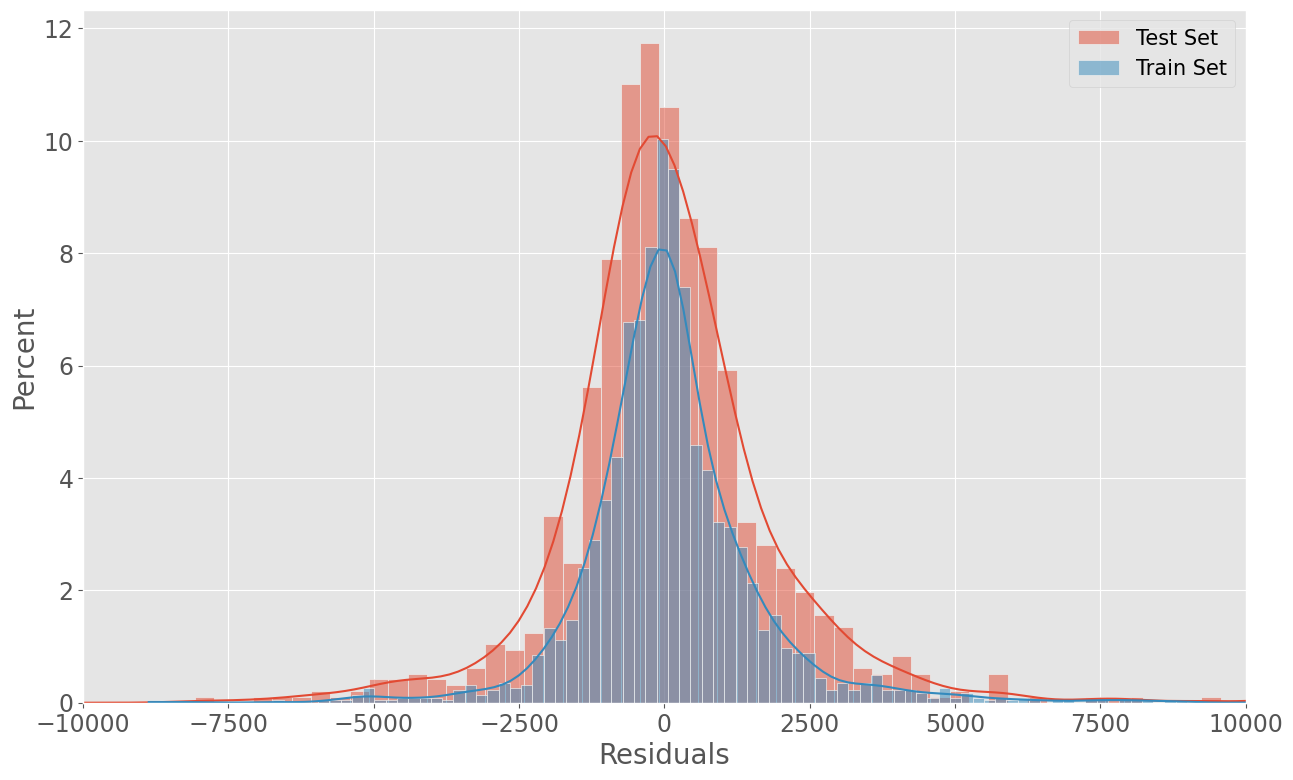
\includegraphics[width=\textwidth]{"content/pics/Distribution_Residuals.png"}
    \caption{.}
    \label{fig:}
\end{figure}

\begin{figure}
\centering
    \makebox[\textwidth][c]{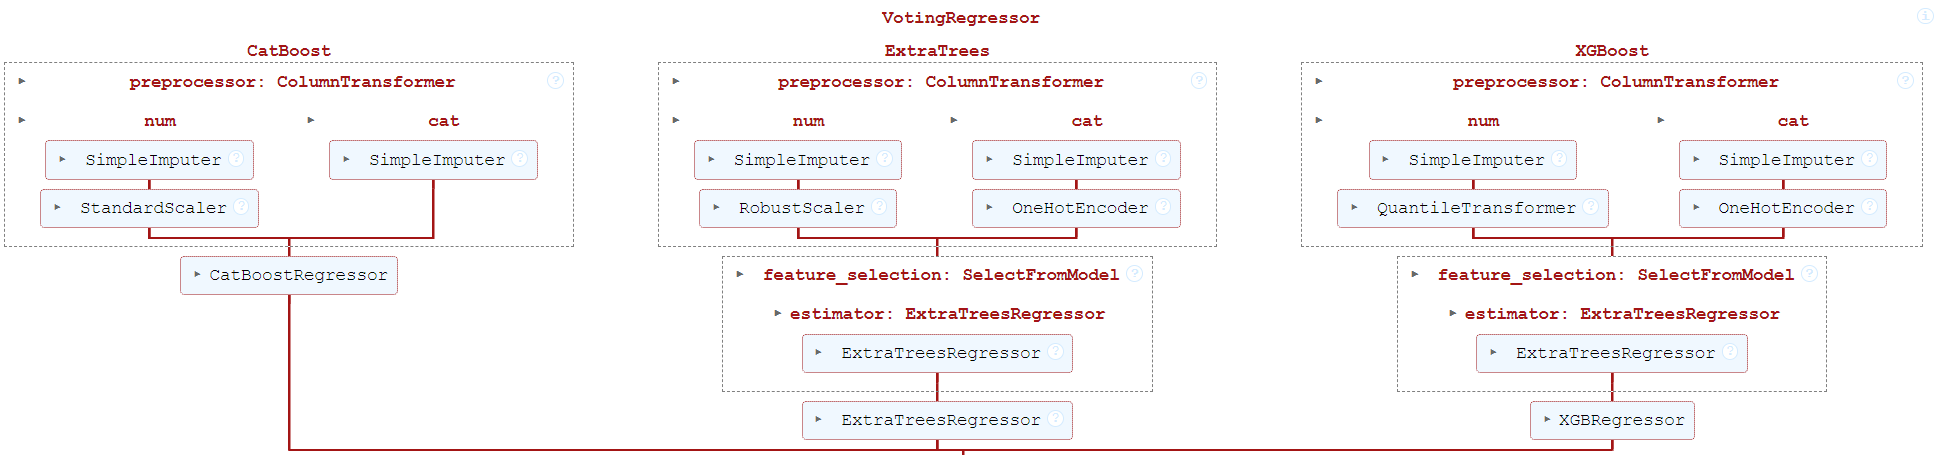
\includegraphics[width=1.25\textwidth]{"content/pics/Ensembled_Model_compromised.png"}}
    \caption{.}
    \label{fig:}
\end{figure}

\begin{figure}
\centering
    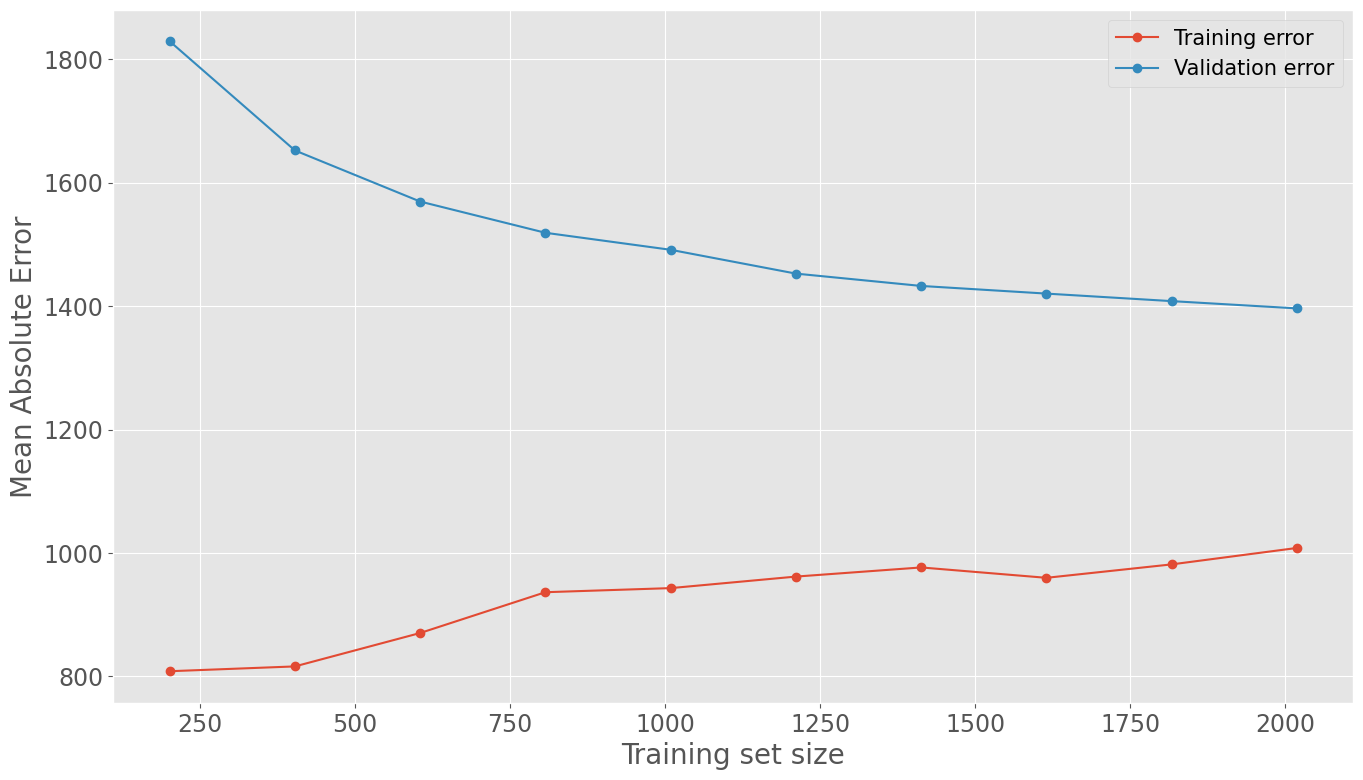
\includegraphics[width=0.8\textwidth]{"content/pics/Learning_curve.png"}
    \caption{.}
    \label{fig:}
\end{figure}

\begin{figure}
\centering
    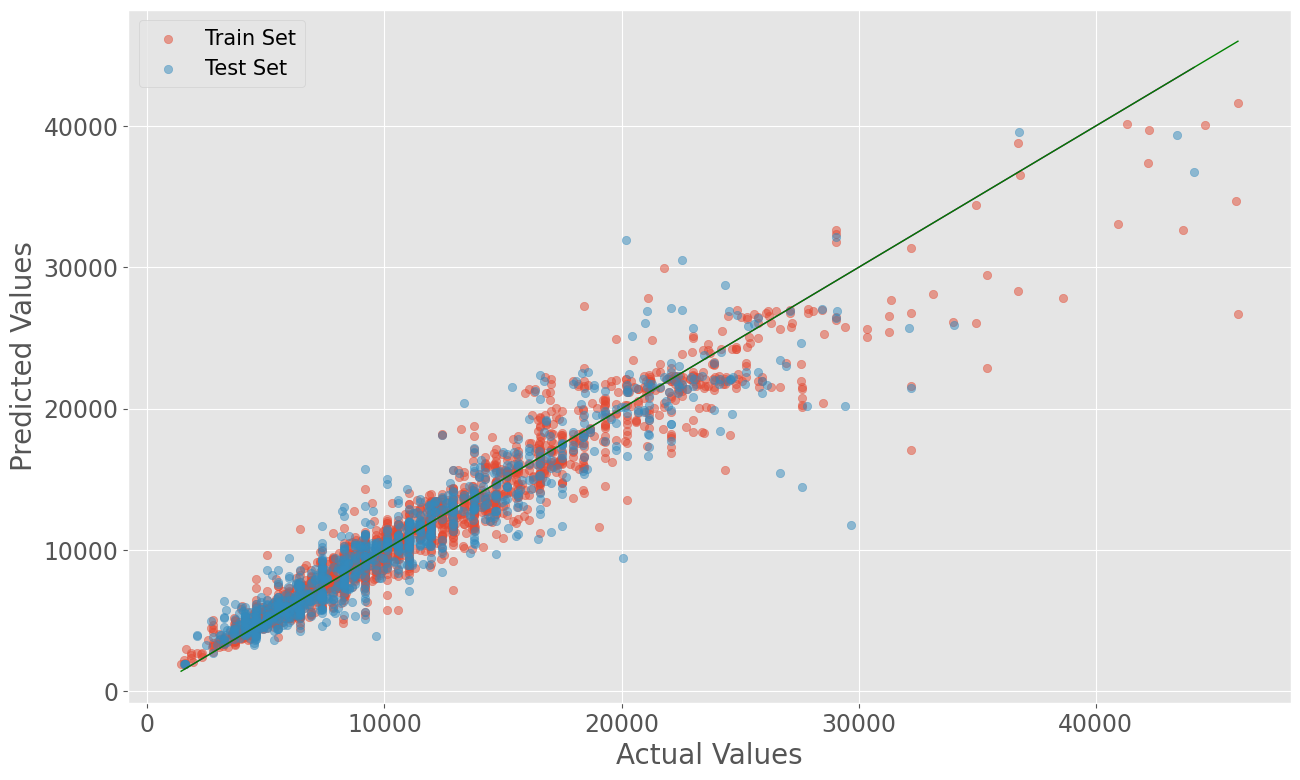
\includegraphics[width=0.8\textwidth]{"content/pics/Predictionerrorplot.png"}
    \caption{.}
    \label{fig:}
\end{figure}



\begin{figure}
\centering
    \makebox[\textwidth][c]{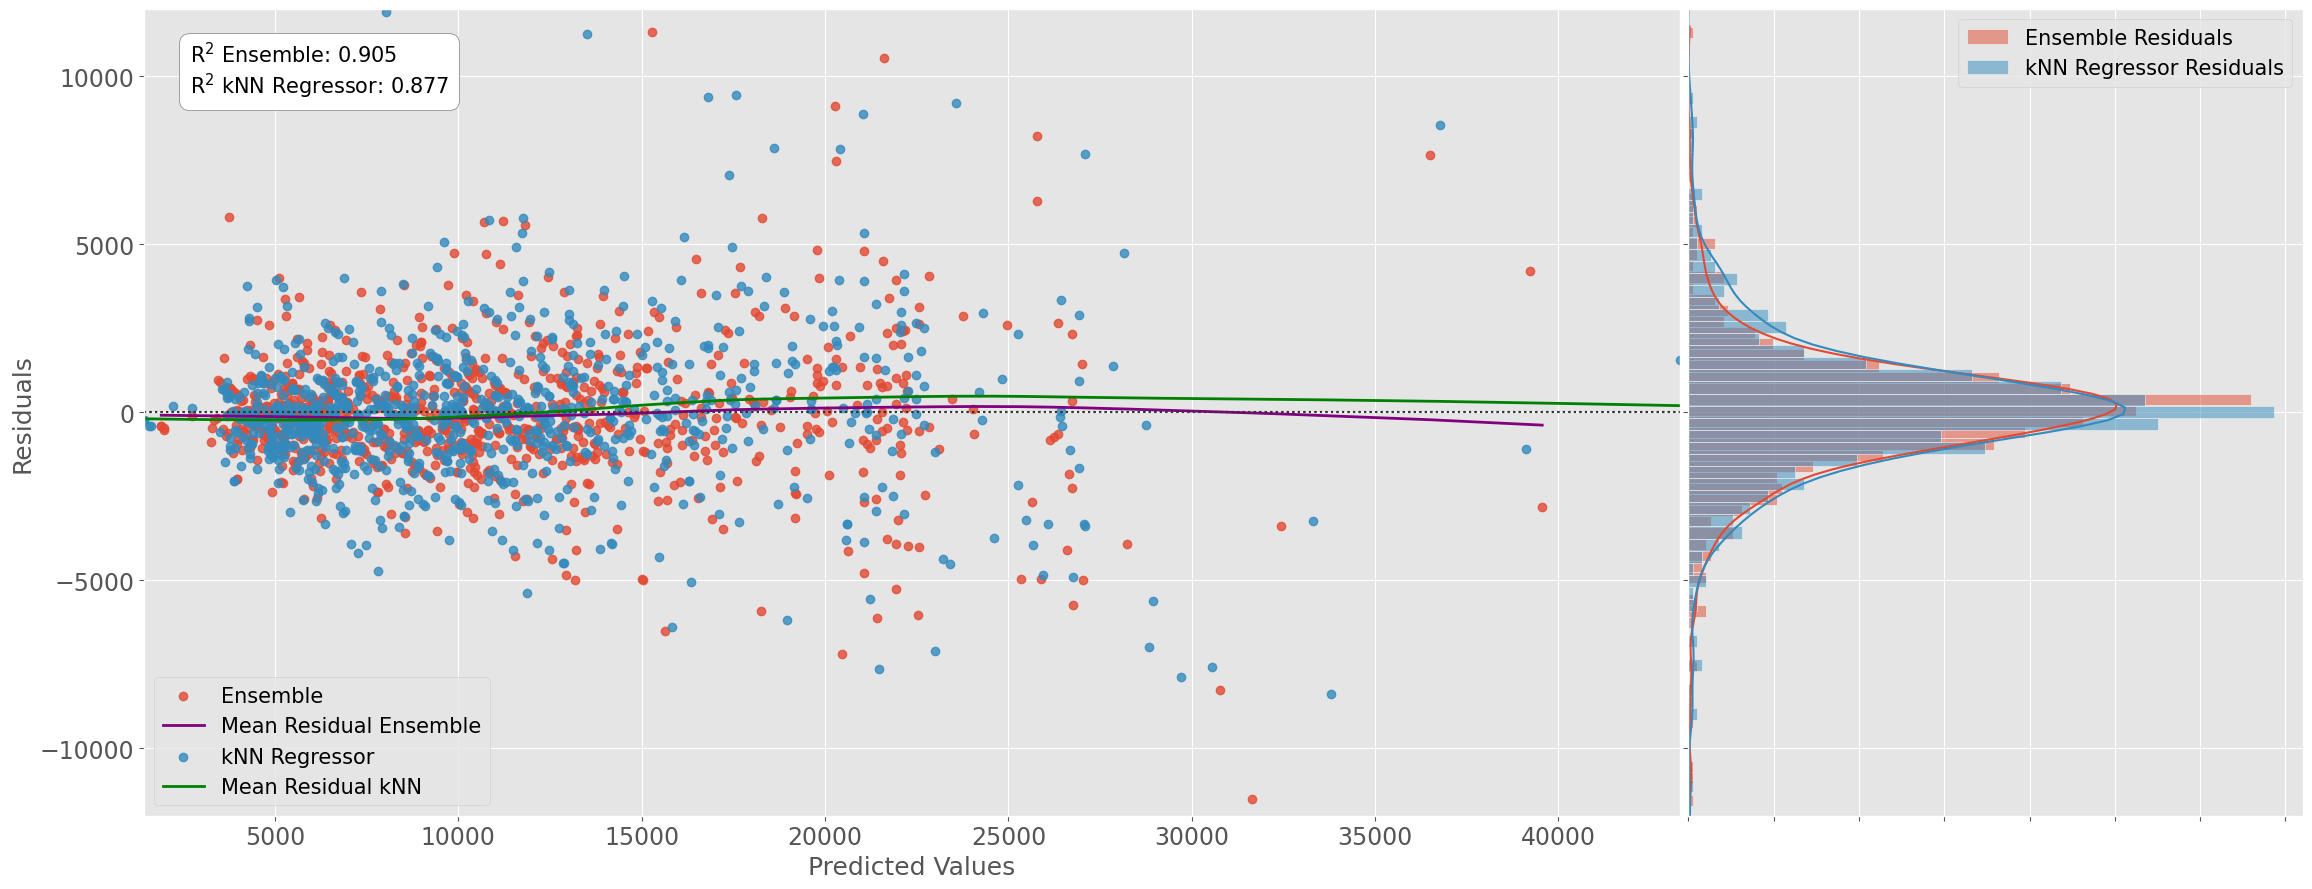
\includegraphics[width=1.25\textwidth]{"content/pics/residuals_Ensemble_kNN.png"}}
    \caption{.}
    \label{fig:}
\end{figure}



\begin{figure}
\centering
    \makebox[\textwidth][c]{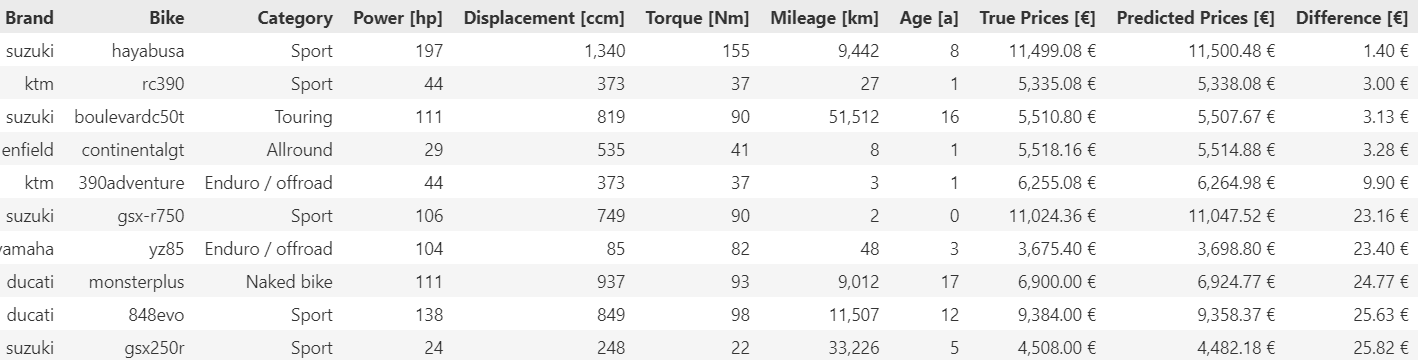
\includegraphics[width=1.35\textwidth]{"content/pics/Table_Best.png"}}    
    \caption{.}
    \label{fig:}
\end{figure}

\begin{figure}
\centering
    \makebox[\textwidth][c]{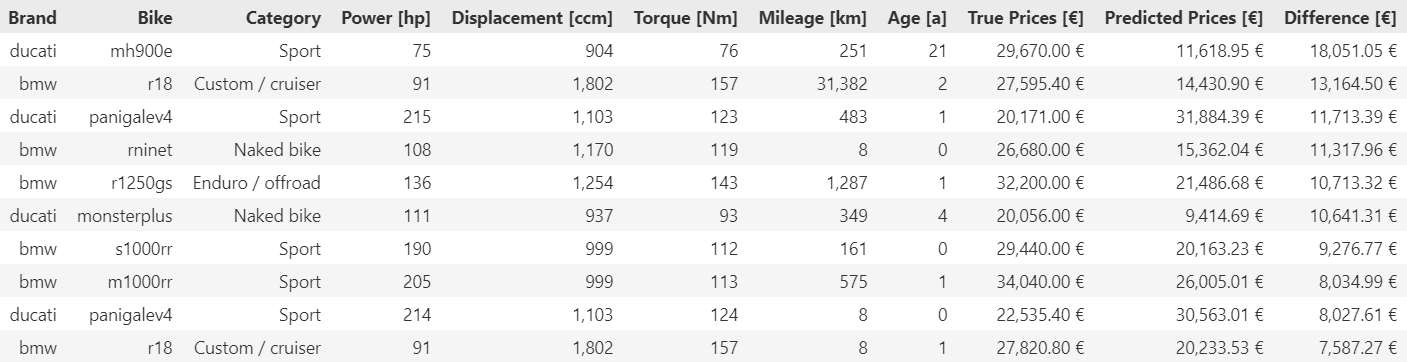
\includegraphics[width=1.35\textwidth]{"content/pics/Table_Worst.png"}}
    \caption{.}
    \label{fig:}
\end{figure}